\chapter{Appendix}
\section{Class Diagrams}
\label{appendix:class_diagrams}
\begin{figure}[h]
\centerline{\includegraphics[scale=0.36]{ClientProject} }
\caption{Client diagram}
\end{figure}
\newpage
\begin{figure}[h]
\centerline{\includegraphics[scale=0.8]{GameDataProject} }
\caption{Game Data diagram}
\end{figure}
\newpage
\begin{figure}[h]
\centerline{\includegraphics[scale=0.36]{GameProject} }
\caption{Game diagram}
\end{figure}
\newpage
\begin{figure}[h]
\centerline{\includegraphics[scale=0.25]{GameServicesProject} }
\caption{Game Services diagram}
\end{figure}
\newpage
\begin{figure}[h]
\centerline{\includegraphics[scale=0.45]{GeneralServicesProject} }
\caption{General Services diagram}
\end{figure}
\newpage
\begin{figure}[h]
\centerline{\includegraphics[scale=0.43]{SecurityTokenServicesProject} }
\caption{Security Token Services diagram}
\end{figure}
\newpage
\begin{figure}[h]
\centerline{\includegraphics[scale=0.36]{ServerProject} }
\caption{Server diagram}
\end{figure}

\section{SOLID}
\label{appendix:SOLID}
There are 5 principles to SOLID:
\\
\\
\textbf{Single Responsibility Principle (SRP)}
\\
 “There should never be more than one reason for a class to change.”\footnote{srp.pdf, 02/2002, Robert C. Martin, page 1}
\\
\\
This principle focus on cohesion, and means that a class should only be assigned one responsibility, by splitting a class that has multiple responsibilities into different classes. This will allow for good maintainability, since if later some requirements changes, that would mean a change in responsibility amongst the classes as well.
\\
\\
\textbf{Open/Closed Principle (OCP)}
\\
"Software entities (classes, modules, functions, etc.) should be open for extension, but closed for modification."\footnote{ocp.pdf, 01/1996, Robert C. Martin, page 1}
\\
\\
The principle means that we should write our software entities to be extended without modifying the code. This will be achieved by abstraction, since it allows us to change what the software entity does, without changing the code.
\\
\\
\textbf{Liskov Substitution Principle (LSP)}
\\
"Subclasses should be substitutable for their base classes."\footnote{Principles\_and\_Patterns.pdf, 01/2000, Robert C. Martin, page 8}
\\
\\
This means that a subclass of the base class should still function properly, even if a derived class of the base class is passed to it. A violation of LSP, will also result in a violation of OCP.\footnote{Principles\_and\_Patterns.pdf, 01/2000, Robert C. Martin, page 12}
\\
\\
\textbf{Interface Segregation Principle (ISP)}
\\
"Many client specific interfaces are better than one general purpose interface."\footnote{Principles\_and\_Patterns.pdf, 01/2000, Robert C. Martin, page 14}
\\
\\
This means that we should create specific interfaces for each client and inherit multiple of them, instead of one class with all the methods a client would need.
This does not mean that every class that has a service, should have a special interface. Clients should instead be categorized by their type, and then create interfaces for each type. Then if different client types need the same method, it should be added to their interface.\footnote{Principles\_and\_Patterns.pdf, 01/2000, Robert C. Martin, page 15}
\\
\\
\textbf{Dependency Inversion Principle (DIP)}
\\
"Depend upon Abstractions. Do not depend upon concretions."\footnote{Principles\_and\_Patterns.pdf, 01/2000, Robert C. Martin, page 12}
\\
This means that every dependency should be on an interface or an abstract class, not a concrete class or function.
\\
\newpage
\section{GRASP}
There are 9 patterns to GRASP\footnote{Applying UML and patterns, Larman 2005}:
\\
\\
\textbf{Controller}
\\
Controller pattern is used to create a non-UI class that can represent more than one use case. An example of this could be create user and delete user which would have a single controller together.
\\
\\
\textbf{Creator}
\\
The creator pattern uses one class to create other classes in cases where the creator monitors or uses the class it creates. It can have the initialization information for the class and passes it on when the class is created.
\\
\\
\textbf{High Cohesion}
\\
High cohesion is a pattern that attempts to keep objects manageable and understandable. This is achieved by breaking programs into smaller classes and subsystems. If the system is a low cohesion the code can be hard to reuse, maintain and averse to change.
\\
\\
\textbf{Indirection}
\\
Indirection pattern is a low coupling pattern. It takes the mediation between two classes and give them to an intermediate object. An example of this is the introduction of a controller for meditation between data and its representation.
\\
\\
\textbf{Information Expert}
\\
Information expert is a principle is used to delegate responsibilities. Responsibilities includes methods, computed files, and so on. A common use is to look what information is needed to complete it and then determine where that information is stored.
\\
\\
\textbf{Low Coupling}
\\
Low coupling is how much an object have knowledge, relies on and connected to other elements. The low coupling pattern is used to assign the responsibilities to support: low dependency, higher reuse potential and change in one class does not have a big impact on other classes.
\\
\\
\textbf{Polymorphism}
\\
If it is needed to handle alternatives based on a type, polymorphism should be used. An example of this would be if there was two types Dog and Cat, they are both just alternatives to each other. Instead polymorphism should be used, which results in creating a common type Animal, where Dog and Cat are its alternatives by extending or implementing depending on the type.
\\
\\
\textbf{Protected Variations}
\\
This pattern is similar to the Open/Closed principle of SOLID, and should be used when
a change/variation in the software will or would cause the software to be unstable. This is done by using an interface and polymorphism to wrap the old code instead of modifying it directly.
\\
\\
\textbf{Pure Fabrication}
\\
If the Information Expert fails the Pure Fabrication pattern steps in. This is done by creating a class that does not represent the domain concepts. In other words, if the responsibility assigned by the Information Expert does not meet the high cohesion, create a separate class and assign responsibility to it, so that it results in high cohesion.



\section {UseCase Specification}

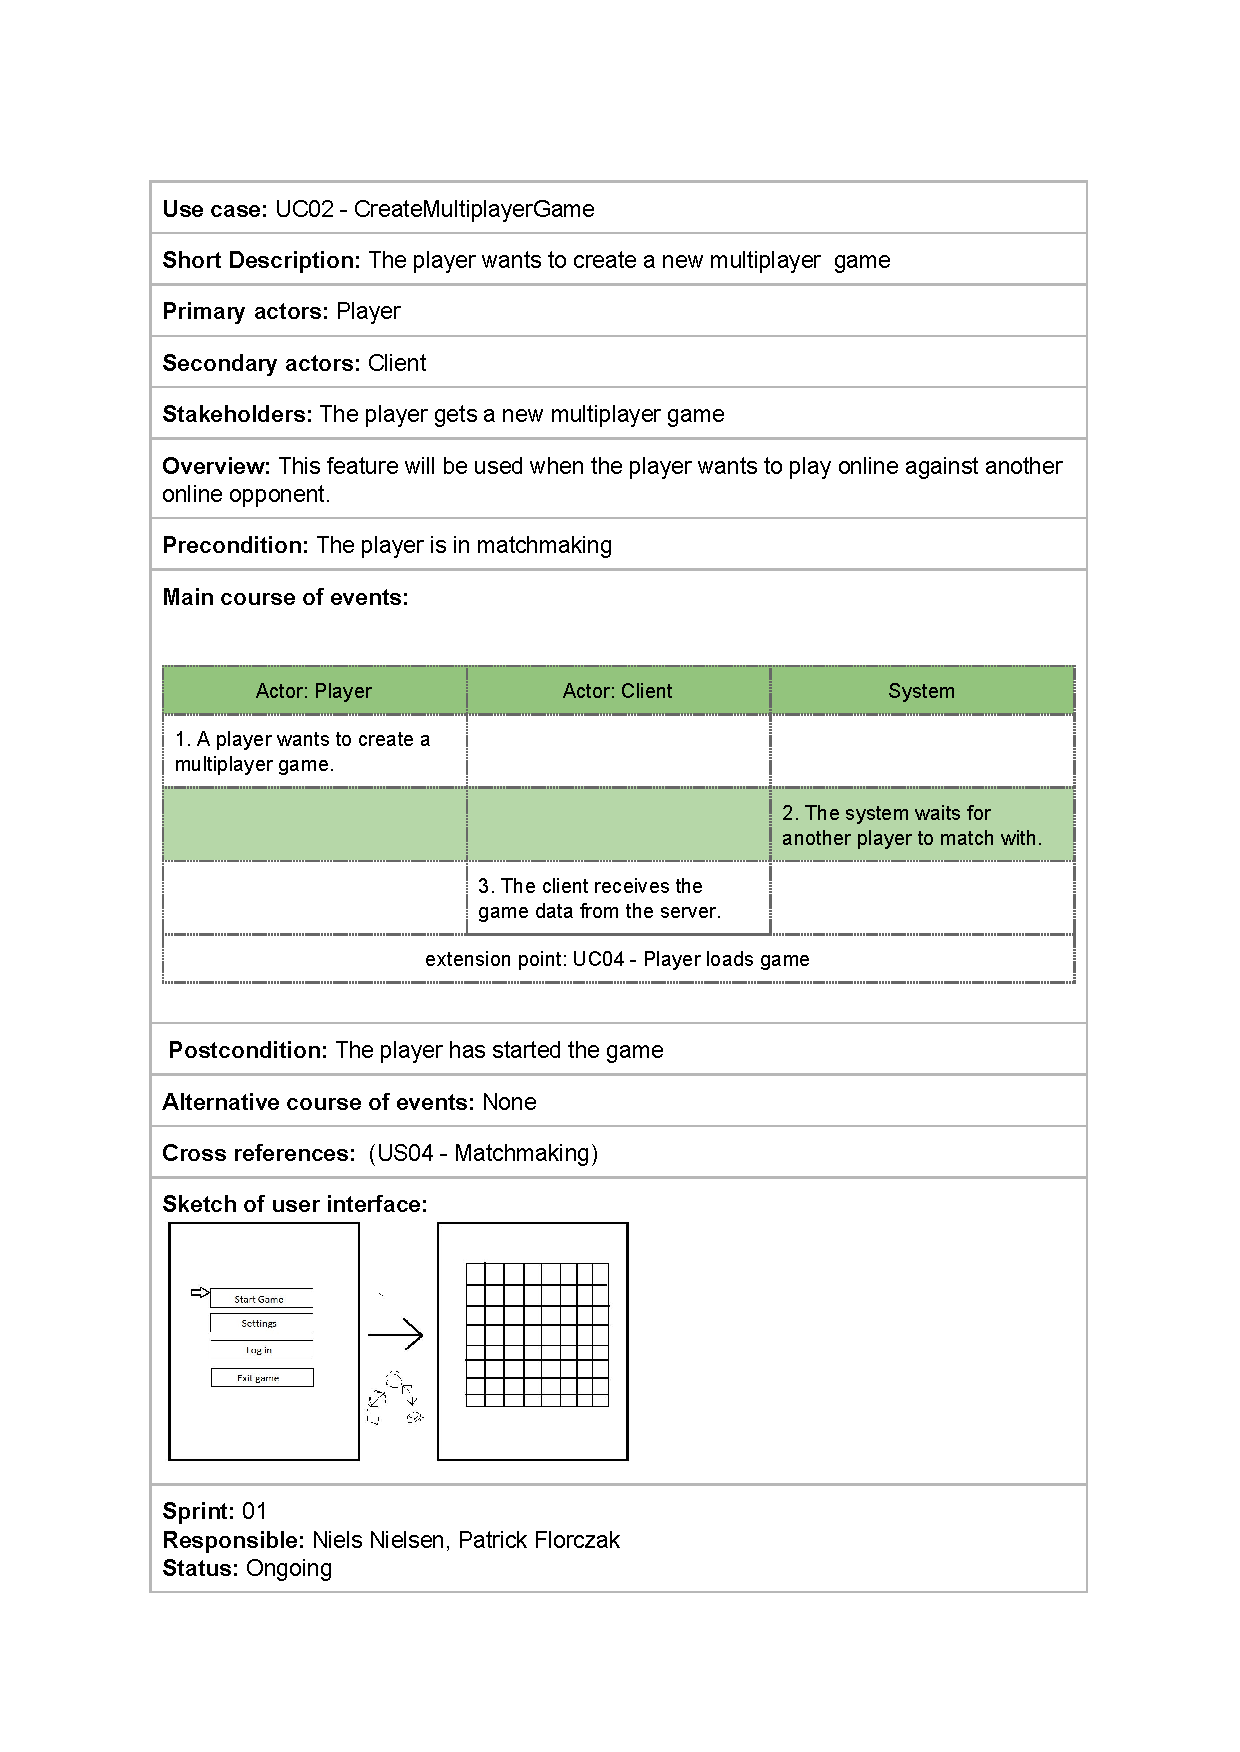
\includepdf[pages=-]{./Images/UseCaseSpecification.pdf}
